\documentclass[]{article}
\usepackage{float}
\usepackage[]{graphicx}
\usepackage{epstopdf} %eps to pdf conversion with same compiler (goes after graphicx!)
\usepackage[]{subcaption}
\captionsetup[figure]{labelfont={bf,footnotesize},textfont=footnotesize}
\captionsetup[table]{labelfont={bf,footnotesize},textfont=footnotesize}
\usepackage{xcolor}
\usepackage{listings}
\lstset{
  frame=single,
  breaklines=true,
  postbreak=\raisebox{0ex}[0ex][0ex]{\ensuremath{\color{red}\hookrightarrow\space}}
}
\usepackage{hyperref}
\usepackage[]{amsmath}

\newcommand{\TwoRowCell}[2][c]{%
\begin{tabular}[#1]{@{}c@{}}#2\end{tabular}}

\title{Simulation - Assignment 3}
\author{Anton Roth}
\date{\today}

\begin{document}
\begin{titlepage}
  \maketitle
  \thispagestyle{empty}
\end{titlepage}

\section*{Implementation}
All tasks have been solely implemented in {\it Matlab}. Files \textit{main\_ga.m} and \textit{tsp\_ga.m} contain the implementations.

The implemented parts of the {\it Genetic Algorithm} (GA) were cross-checked individually for satisfactory behaviour.
The GA was validated through the following two tests:
\begin{enumerate}
  \item Fitness value decreasing with increasing number of generations.
  \item Fitness value decreasing with increasing population size.
\end{enumerate}
The test were performed on the tour with 48 cities and the simulation parameters given in the assignment instructions.
The results are presented in Table \ref{tab:val1} and \ref{tab:val2}.
\begin{table}[H]
  \centering
  \caption{Fitness value vs. increasing number of generations. The population size was set to 100.}
  \begin{tabular}{|c|c|}
    \hline \\
    Number of generations & Fitness value \\ \hline
    100 & 100000 \\ \hline
    1000 & 60000 \\ \hline
    2000 & 50000 \\ \hline
  \end{tabular}
  \label{tab:val1}
\end{table}

\begin{table}[H]
  \centering
  \caption{Fitness value vs. increasing population size. The number of generations was set to 1000.}
  \begin{tabular}{|c|c|}
    \hline \\
    Population size & Fitness value \\ \hline
    10 & 140000 \\ \hline
    50 & 65000 \\ \hline
    200 & 50000 \\ \hline
  \end{tabular}
  \label{tab:val2}
\end{table}

It was noted that the implemented GA did not perform as well as the algorithm used in lab 3.
For a population size of 100 and 1000 generations it reached a fitness value of 34000 (cf. 60000 for this GA).
This is troubling.
However, it can be due to many reasons.
For instance:
\begin{itemize}
  \item The simulation parameters in this GA might not be as optimised as in the other GA.
  \item The GA implementation itself might not be as optimal as in the other GA.
\end{itemize}


\section*{Task 1}
The results of the simulations are presented in Figure \ref{fig:task1}.

\begin{figure}[H]
  \begin{subfigure}{0.5\textwidth}
     \centering
     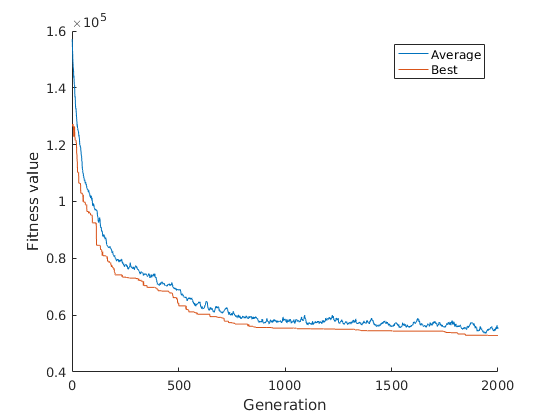
\includegraphics[width=0.99\linewidth]{../GA_TSP/t148.png}
     \caption{48 cities.}
     \label{sfig:t148}
  \end{subfigure}%
  \begin{subfigure}{0.5\textwidth}
     \centering
     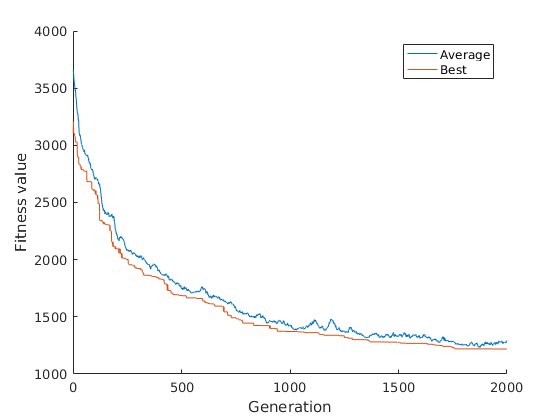
\includegraphics[width=0.99\linewidth]{../GA_TSP/t170.png}
     \caption{70 cities.}
     \label{sfig:t170}
  \end{subfigure}%

  \begin{subfigure}{\textwidth}
     \centering
     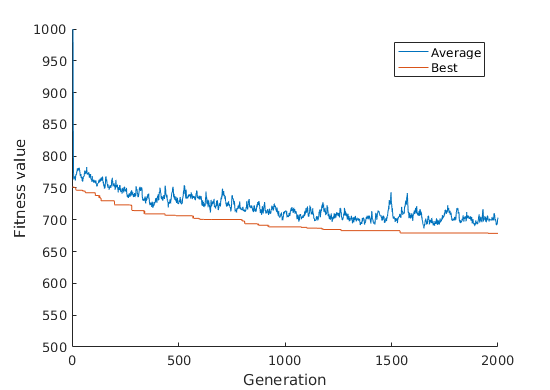
\includegraphics[width=0.5\linewidth]{../GA_TSP/t196.png}
     \caption{96 cities.}
     \label{sfig:t196}
  \end{subfigure}%
  \caption{The implemented GA was run for three different TSPs. The population average and the best fitness value has been plotted vs. the population generation.}
  \label{fig:task1}
\end{figure}

Using these plots, explain the convergence behavior of GA for the three data files (i.e. do they converge? How quickly they converge?).

The fitness, of the population average such as the best in the generation, decreases as the generations pass.
This indicates an improvement of the population in general and the best individual in the population.
The slope of the curves decreases the further along the generations one goes.
Thus, it can be interpreted that the population converges to a certain mix of solutions.

The average fitness follows the trend of the best fitness strictly, but with an added positive shift.
Of course the average should be larger than the minimum of the population.
Interestingly, the curve patterns are, if fluctuations are neglected, almost identical.
This is could be due to the {\it roulette wheel} selection in combination with the elitism which always works to favour the best fitted individuals.

If one compares the three simulations it can be observed that the convergence is the fastest for the 96 city TSP.
The convergence is very similar between the 48 and 70 city TSP, but the 48 city TSP might converge the fastest.
It seems logical that the more cities in the TSP the longer you can be from the optimal solution.
Hence, a more rapid convergence should be pronounced.
However, this is not observed comparing the 48 and 70 city TSPs.
Strange \dots




\section*{Task 2}
The implemented GA was run 15 times for a total number of generations ranging from 100 to 2000 with a step size of 100. For each total number of generation the average of the best fitness value and its upper and lower 95\% confidence limits were calculated.
The 95\% confidence interval was calculated using the normal distribution approximation as:
\begin{equation*}
    [\bar{x} - 1.96\cdot\frac{\sigma}{\sqrt{N}}, \bar{x} + 1.96\cdot\frac{\sigma}{\sqrt{N}}]
  \end{equation*}
Here $x$ is the samples, $\bar{x}$ the estimated mean, $\sigma$ the sample standard deviation and $N$ the number of samples.
The results of the simulation of task 2 is presented in Figure \ref{fig:task2}.

\begin{figure}[H]
  \begin{subfigure}{0.5\textwidth}
     \centering
     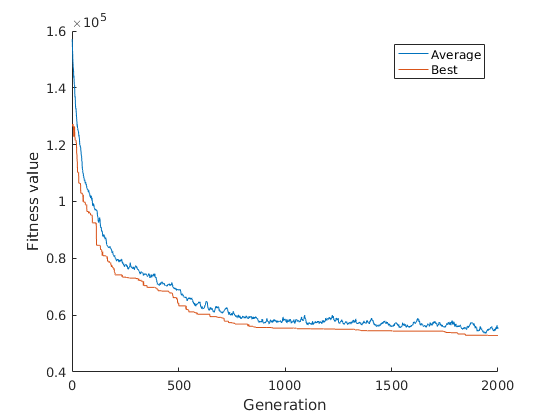
\includegraphics[width=0.99\linewidth]{../GA_TSP/t148.png}
     \caption{48 cities.}
     \label{sfig:t248}
  \end{subfigure}%
  \begin{subfigure}{0.5\textwidth}
     \centering
     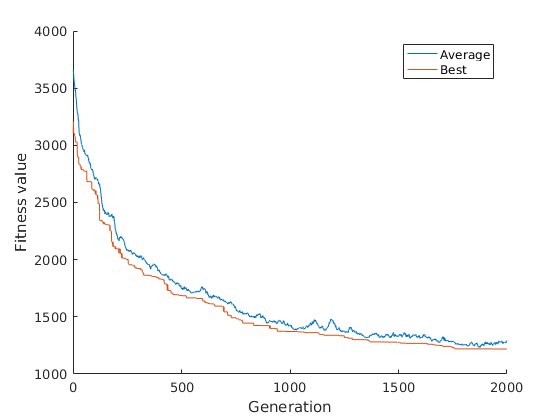
\includegraphics[width=0.99\linewidth]{../GA_TSP/t170.png}
     \caption{70 cities.}
     \label{sfig:t270}
  \end{subfigure}%

  \begin{subfigure}{\textwidth}
     \centering
     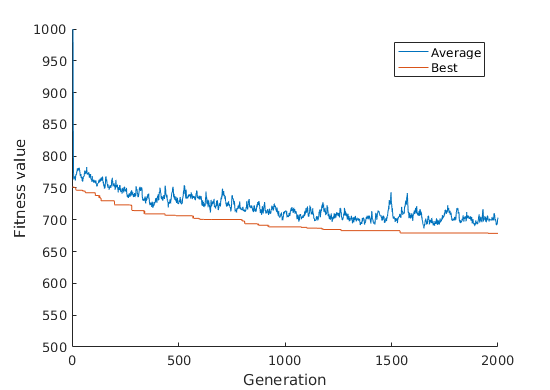
\includegraphics[width=0.5\linewidth]{../GA_TSP/t196.png}
     \caption{96 cities.}
     \label{sfig:t296}
  \end{subfigure}%
  \caption{The average of the best fitness value with its upper and lower 95\% confidence limits for the 20 different total number of generations (x-axis). For the three different TSPs.}
  \label{fig:task2}
\end{figure}

r96.  By observing . Do this your experiment plots, explain separately the for convergence the three data behavior files of loadatt48, GA for each loadst70,
 data
 file scenario and with respect to
  . For which data file the confidence interval is tighter
  and what does this mean?

What is clearly observed in each of the plots is the improvement of the final value of the GA algorithm with increasing total number of generations simulated.
This is expected since the roulette wheel selection and the elitism works to always keep the best solutions in the population.
The crossover and the mutation enables the improvement.
The improvement can be observed to be the largest for a smaller total number of generations simulated.
It can be explained by that there is always the largest potential improvement of the first generation while it decreases as generations pass.



\end{document}

